\documentclass[aspectratio=169,11pt]{ctexbeamer}

\usetheme{Madrid}
\usecolortheme{default}
\setbeamertemplate{navigation symbols}{}
\setbeamertemplate{footline}[frame number]

\usepackage{amsmath}
\usepackage{booktabs}
\usepackage{graphicx}
\usepackage{tikz}
\usetikzlibrary{arrows.meta,positioning,shapes.geometric,shapes.misc}

\graphicspath{{../figures/}{figures/}}

\definecolor{mainblue}{RGB}{31,87,140}
\definecolor{accentred}{RGB}{190,60,47}
\definecolor{softgray}{RGB}{245,247,250}
\definecolor{darkgreen}{RGB}{31,120,82}

\setbeamercolor{title}{fg=mainblue}
\setbeamercolor{frametitle}{fg=mainblue}
\setbeamercolor{block title}{bg=mainblue,fg=white}
\setbeamercolor{block body}{bg=softgray,fg=black}

\title{Reproduction: Stealing ML Models via Prediction APIs}
\subtitle{Python 3 本地黑盒 oracle 复现}
\author{Model-Stealing-Reproduce-Pre}
\date{}

\newcommand{\good}[1]{\textcolor{darkgreen}{#1}}
\newcommand{\warn}[1]{\textcolor{accentred}{#1}}
\newcommand{\code}[1]{\texttt{#1}}

\begin{document}

\begin{frame}
  \titlepage
\end{frame}

\begin{frame}{复现目标：不是跑旧代码，而是复现攻击机制}
  \begin{columns}[T,onlytextwidth]
    \begin{column}{0.50\textwidth}
      \begin{block}{本地黑盒设置}
        \begin{itemize}
          \item 本地训练受害者模型 $f$
          \item 攻击者只能访问 query API
          \item 不读取模型参数、不访问训练集
          \item 得到副本 $f' \approx f$
        \end{itemize}
      \end{block}
      \vspace{0.4em}
      \begin{block}{为什么这样复现？}
        原仓库是 Python 2 + 旧 sklearn + Theano + AWS/BigML wrapper。\\
        我们把论文核心攻击抽象成 Python 3 的本地 oracle，便于讲解和现场演示。
      \end{block}
    \end{column}
    \begin{column}{0.46\textwidth}
      \centering
      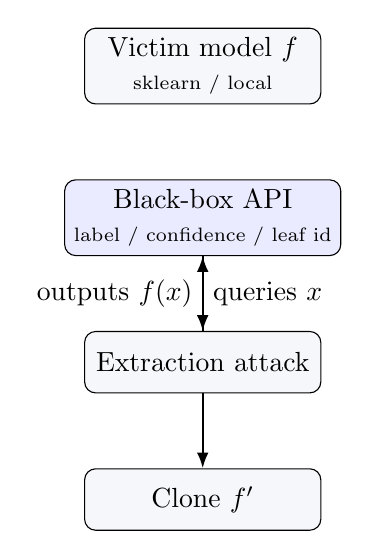
\begin{tikzpicture}[
        node distance=0.95cm,
        box/.style={draw, rounded corners, minimum width=3.0cm, minimum height=0.78cm, align=center, fill=softgray},
        api/.style={draw, rounded corners, minimum width=3.1cm, minimum height=0.78cm, align=center, fill=blue!8},
        arr/.style={-{Latex[length=2mm]}, thick}
      ]
        \node[box] (target) {Victim model $f$\\\scriptsize sklearn / local};
        \node[api, below=of target] (api) {Black-box API\\\scriptsize label / confidence / leaf id};
        \node[box, below=of api] (attack) {Extraction attack};
        \node[box, below=of attack] (clone) {Clone $f'$};
        \draw[arr] (attack) -- node[right]{queries $x$} (api);
        \draw[arr] (api) -- node[left]{outputs $f(x)$} (attack);
        \draw[arr] (attack) -- (clone);
      \end{tikzpicture}
    \end{column}
  \end{columns}
\end{frame}

\begin{frame}{复现实验总览：数据集、模型、攻击接口}
  \small
  \begin{tabular}{llll}
    \toprule
    Phase & 数据集 & 受害者模型 & 攻击接口 \\
    \midrule
    Binary LR & Breast Cancer & Logistic Regression & \code{query\_proba} \\
    Multiclass LR & Iris / Digits & Softmax / OvR LR & \code{query\_proba} \\
    Rounding & Digits & Softmax / OvR LR & rounded \code{query\_proba} \\
    Decision Tree & Iris & DecisionTree(max\_depth=3) & \code{query\_leaf\_id} \\
    Label-Only & Digits & Softmax LR & \code{query\_label} \\
    KLR leakage & Digits & RBF representer model & extracted white-box params \\
    \bottomrule
  \end{tabular}
  \vspace{1.0em}

  \begin{block}{统一评估}
    \begin{itemize}
      \item \textbf{Test agreement}: 测试集上 $f'(x)=f(x)$ 的比例
      \item \textbf{Uniform agreement}: 在 $[-1,1]^d$ 均匀采样点上的一致率
      \item \textbf{TV distance}: 比较概率分布时使用 total variation distance
    \end{itemize}
  \end{block}
\end{frame}

\begin{frame}{Equation-Solving：confidence 把分类变成解方程}
  \begin{columns}[T,onlytextwidth]
    \begin{column}{0.52\textwidth}
      \begin{block}{二元 Logistic Regression}
        \[
          p = \sigma(w^\top x + b)
        \]
        \[
          \log\frac{p}{1-p} = w^\top x + b
        \]
        \begin{itemize}
          \item Breast Cancer: $d=30$
          \item 未知数：$w_1,\dots,w_{30},b$
          \item 查询 $d+1=31$ 个线性无关点
          \item 解线性系统 $[X,1]\theta=\mathrm{logit}(p)$
        \end{itemize}
      \end{block}
    \end{column}
    \begin{column}{0.44\textwidth}
      \centering
      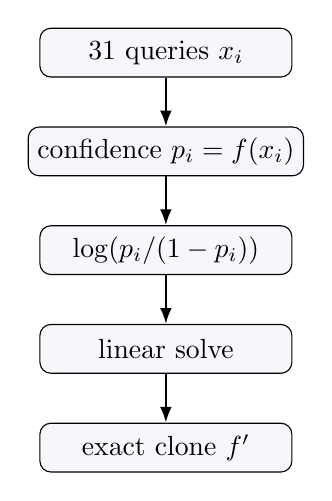
\begin{tikzpicture}[
        node distance=0.62cm,
        box/.style={draw, rounded corners, align=center, fill=softgray, minimum width=3.2cm, minimum height=0.62cm},
        arr/.style={-{Latex[length=2mm]}, thick}
      ]
        \node[box] (q) {31 queries $x_i$};
        \node[box, below=of q] (p) {confidence $p_i=f(x_i)$};
        \node[box, below=of p] (eq) {$\log(p_i/(1-p_i))$};
        \node[box, below=of eq] (solve) {linear solve};
        \node[box, below=of solve] (clone) {exact clone $f'$};
        \draw[arr] (q) -- (p);
        \draw[arr] (p) -- (eq);
        \draw[arr] (eq) -- (solve);
        \draw[arr] (solve) -- (clone);
      \end{tikzpicture}
    \end{column}
  \end{columns}
\end{frame}

\begin{frame}{Equation-Solving 结果：约 1 query / parameter 即可}
  \begin{columns}[T,onlytextwidth]
    \begin{column}{0.50\textwidth}
      \small
      \begin{tabular}{lrrrr}
        \toprule
        模型 & 参数 & 查询 & Test & Uniform \\
        \midrule
        Binary LR & 31 & 31 & 100\% & 100\% \\
        Iris softmax & 15 & 15 & 100\% & 100\% \\
        Digits softmax & 650 & 650 & 100\% & 100\% \\
        Digits OvR & 650 & 650 & 100\% & 100\% \\
        \bottomrule
      \end{tabular}
      \vspace{1em}
      \begin{block}{讲解重点}
        Digits softmax 的 650 次查询，对应论文 Amazon Digits 案例的量级。这里用本地 oracle 复现了同样的核心现象。
      \end{block}
    \end{column}
    \begin{column}{0.47\textwidth}
      \centering
      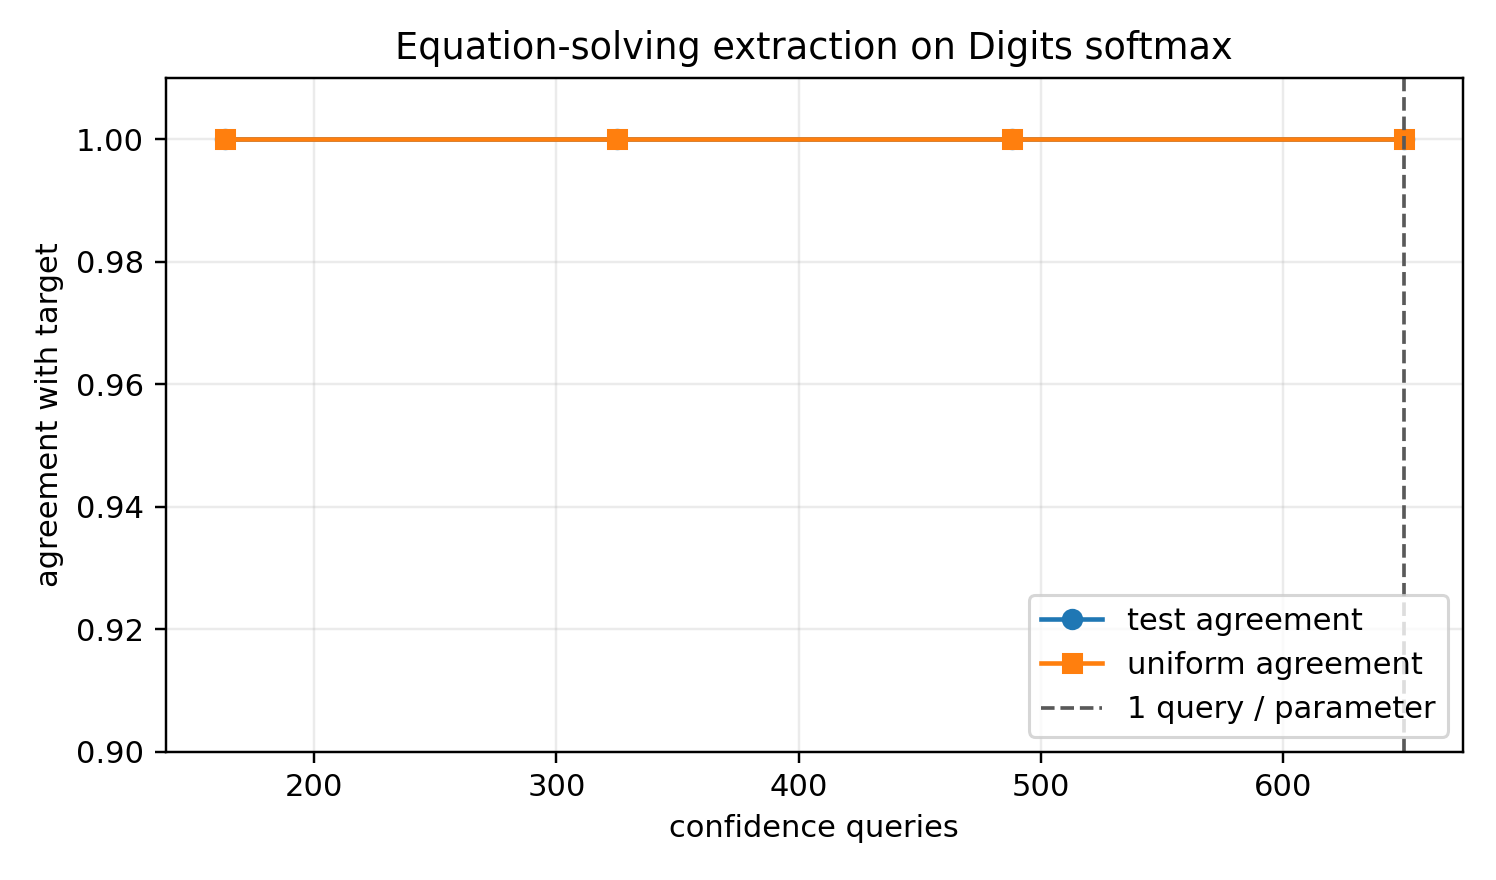
\includegraphics[width=\textwidth]{equation_budget_curve.png}
    \end{column}
  \end{columns}
\end{frame}

\begin{frame}{Rounding 防御：小数位数少了，攻击才明显变难}
  \begin{columns}[T,onlytextwidth]
    \begin{column}{0.43\textwidth}
      \scriptsize
      \begin{tabular}{rrrr}
        \toprule
        小数位 & 查询 & Test & Uniform \\
        \midrule
        5 & 650 & 100.00\% & 99.97\% \\
        4 & 650 & 100.00\% & 99.96\% \\
        3 & 650 & 100.00\% & 99.90\% \\
        2 & 650 & 99.63\% & 99.09\% \\
        \bottomrule
      \end{tabular}
      \vspace{0.5em}
      \begin{block}{结论}
        4--5 位 confidence 基本挡不住；2--3 位会明显增加概率误差，但仍不是完整防御。
      \end{block}
    \end{column}
    \begin{column}{0.54\textwidth}
      \centering
      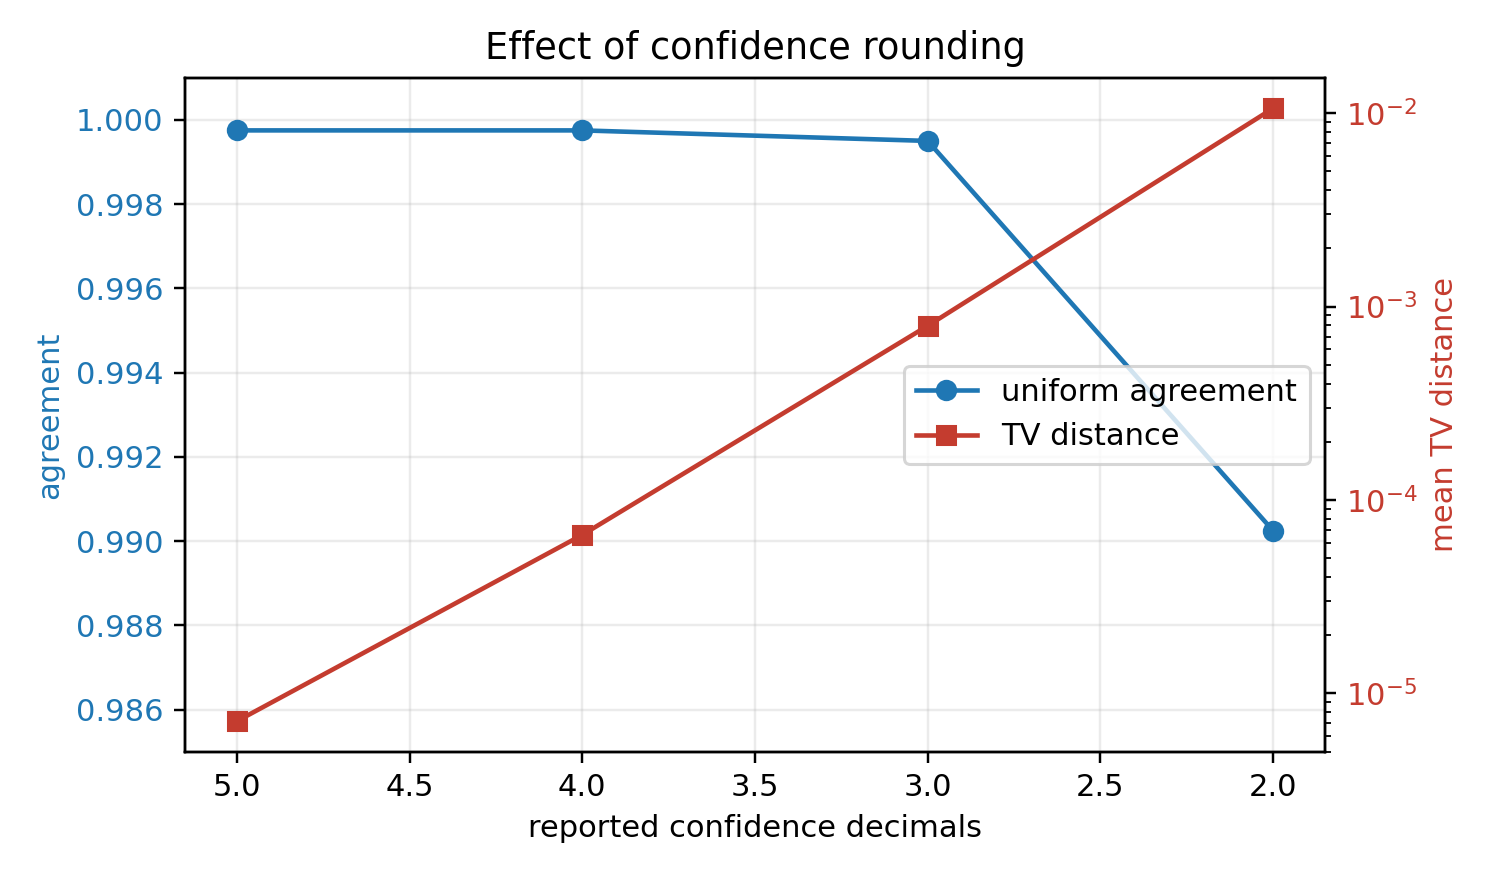
\includegraphics[width=\textwidth]{rounding_curve.png}
    \end{column}
  \end{columns}
\end{frame}

\begin{frame}{Decision Tree：leaf id 是路径“身份证”}
  \begin{columns}[T,onlytextwidth]
    \begin{column}{0.43\textwidth}
      \small
      \begin{block}{攻击步骤}
        \begin{enumerate}
          \item 查询一个点，得到 leaf id
          \item 逐个改变特征值
          \item leaf id 变化 $\Rightarrow$ 路径在该特征上分裂
          \item 连续特征二分搜索阈值
        \end{enumerate}
      \end{block}
      \vspace{-0.4em}
      \scriptsize
      \begin{tabular}{lr}
        \toprule
        指标 & 数值 \\
        \midrule
        Dataset & Iris \\
        Target leaves & 5 \\
        Extracted leaves & 5 \\
        Queries & 557 \\
        Test agreement & 100\% \\
        Uniform agreement & 100\% \\
        \bottomrule
      \end{tabular}
    \end{column}
    \begin{column}{0.55\textwidth}
      \centering
      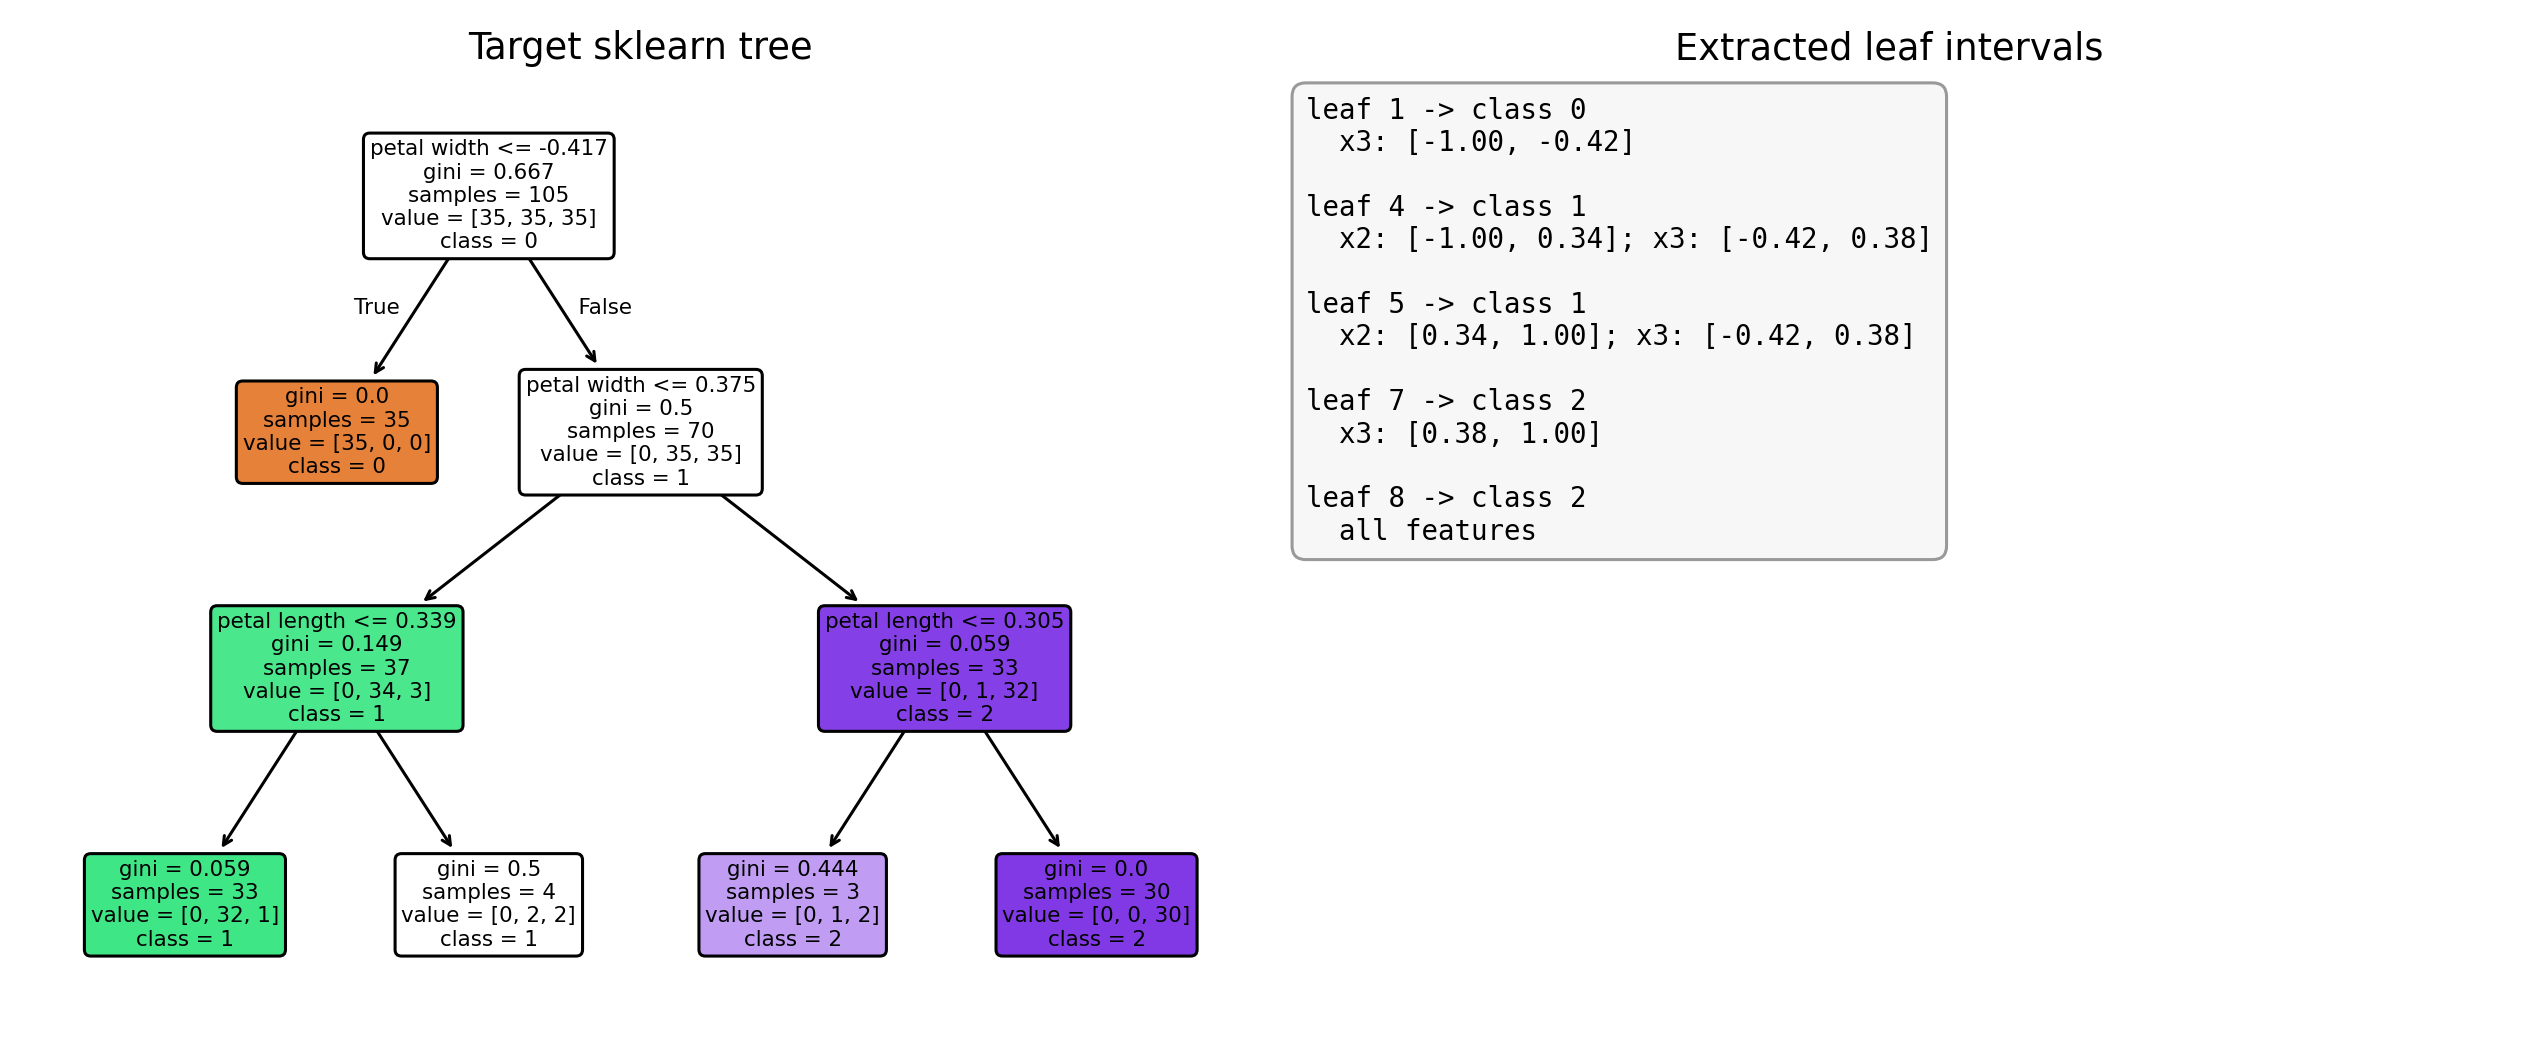
\includegraphics[width=\textwidth]{tree_path_finding.png}
    \end{column}
  \end{columns}
\end{frame}

\begin{frame}{Label-Only：去掉 confidence 后，成本显著上升}
  \begin{columns}[T,onlytextwidth]
    \begin{column}{0.47\textwidth}
      \small
      \begin{tabular}{lrr}
        \toprule
        方法 & 查询 & Uniform agreement \\
        \midrule
        confidence solve & 650 & 100.00\% \\
        label uniform & 650 & 68.83\% \\
        label adaptive & 650 & 76.13\% \\
        label adaptive & 6,500 & 97.83\% \\
        label adaptive & 26,000 & 99.33\% \\
        \bottomrule
      \end{tabular}
      \vspace{1em}
      \begin{block}{讲解重点}
        只返回 label 能有效抬高攻击成本；但主动学习式 retraining 仍能逐步逼近目标模型。
      \end{block}
    \end{column}
    \begin{column}{0.50\textwidth}
      \centering
      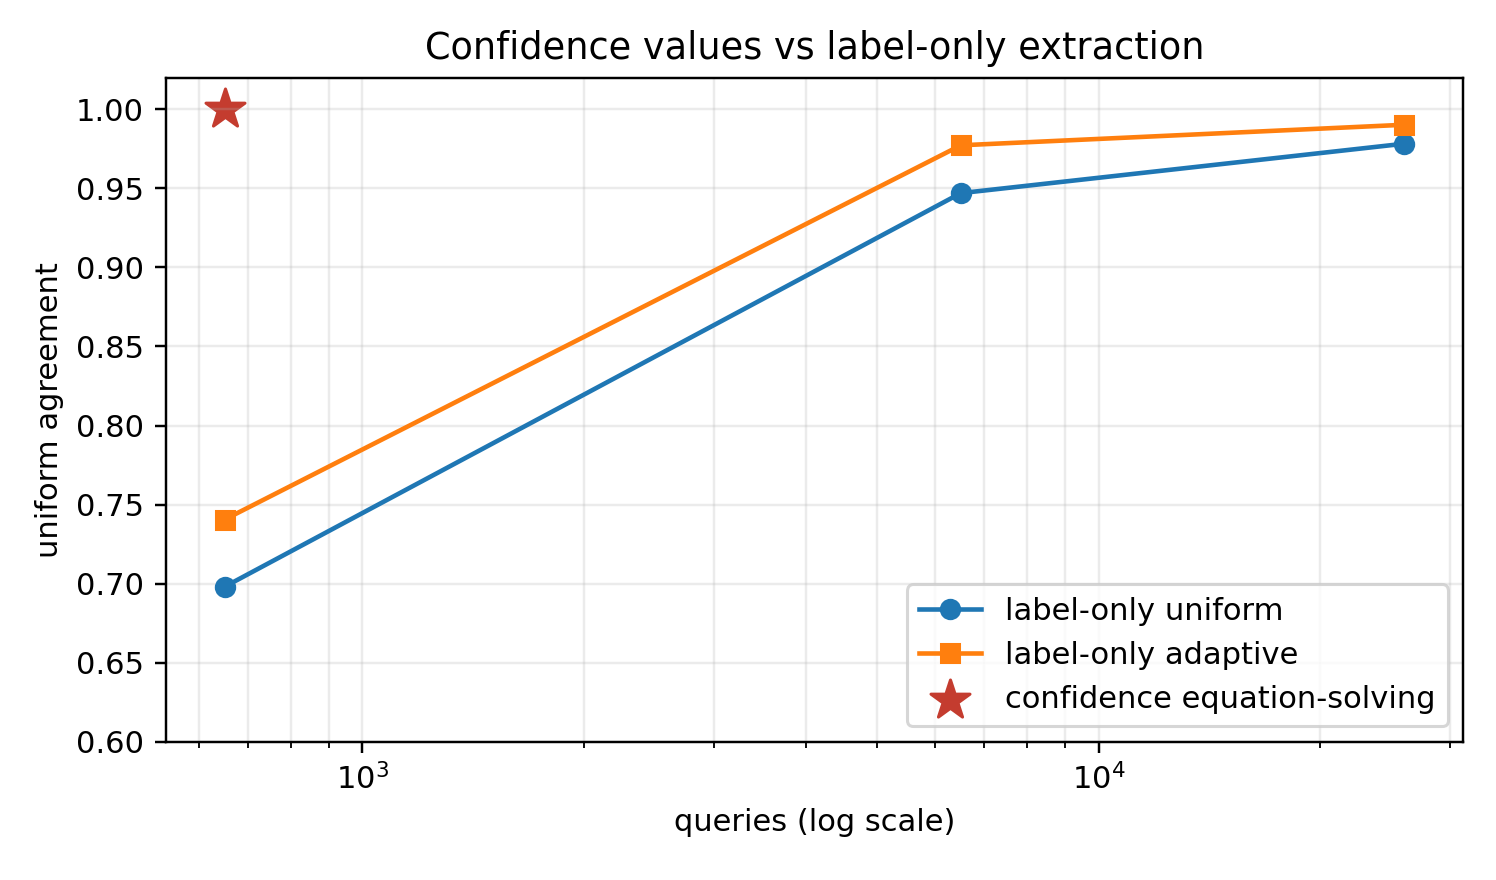
\includegraphics[width=\textwidth]{confidence_vs_label_only.png}
    \end{column}
  \end{columns}
\end{frame}

\begin{frame}{KLR Leakage：模型参数里嵌着训练样本}
  \begin{columns}[T,onlytextwidth]
    \begin{column}{0.42\textwidth}
      \scriptsize
      \begin{block}{教学版 representer model}
        \[
          s_c(x)=\sum_{r:y_r=c}\exp(-\gamma\|x-r\|^2)
        \]
        \begin{itemize}
          \item Digits 数据集
          \item 每类 5 个 representers
          \item 总计 50 张训练图像
          \item 提取白盒模型 $\Rightarrow$ representer 矩阵泄露
        \end{itemize}
      \end{block}
      \begin{block}{要传达的风险}
        模型窃取不只偷走功能，也可能带走训练数据子集。
      \end{block}
    \end{column}
    \begin{column}{0.55\textwidth}
      \centering
      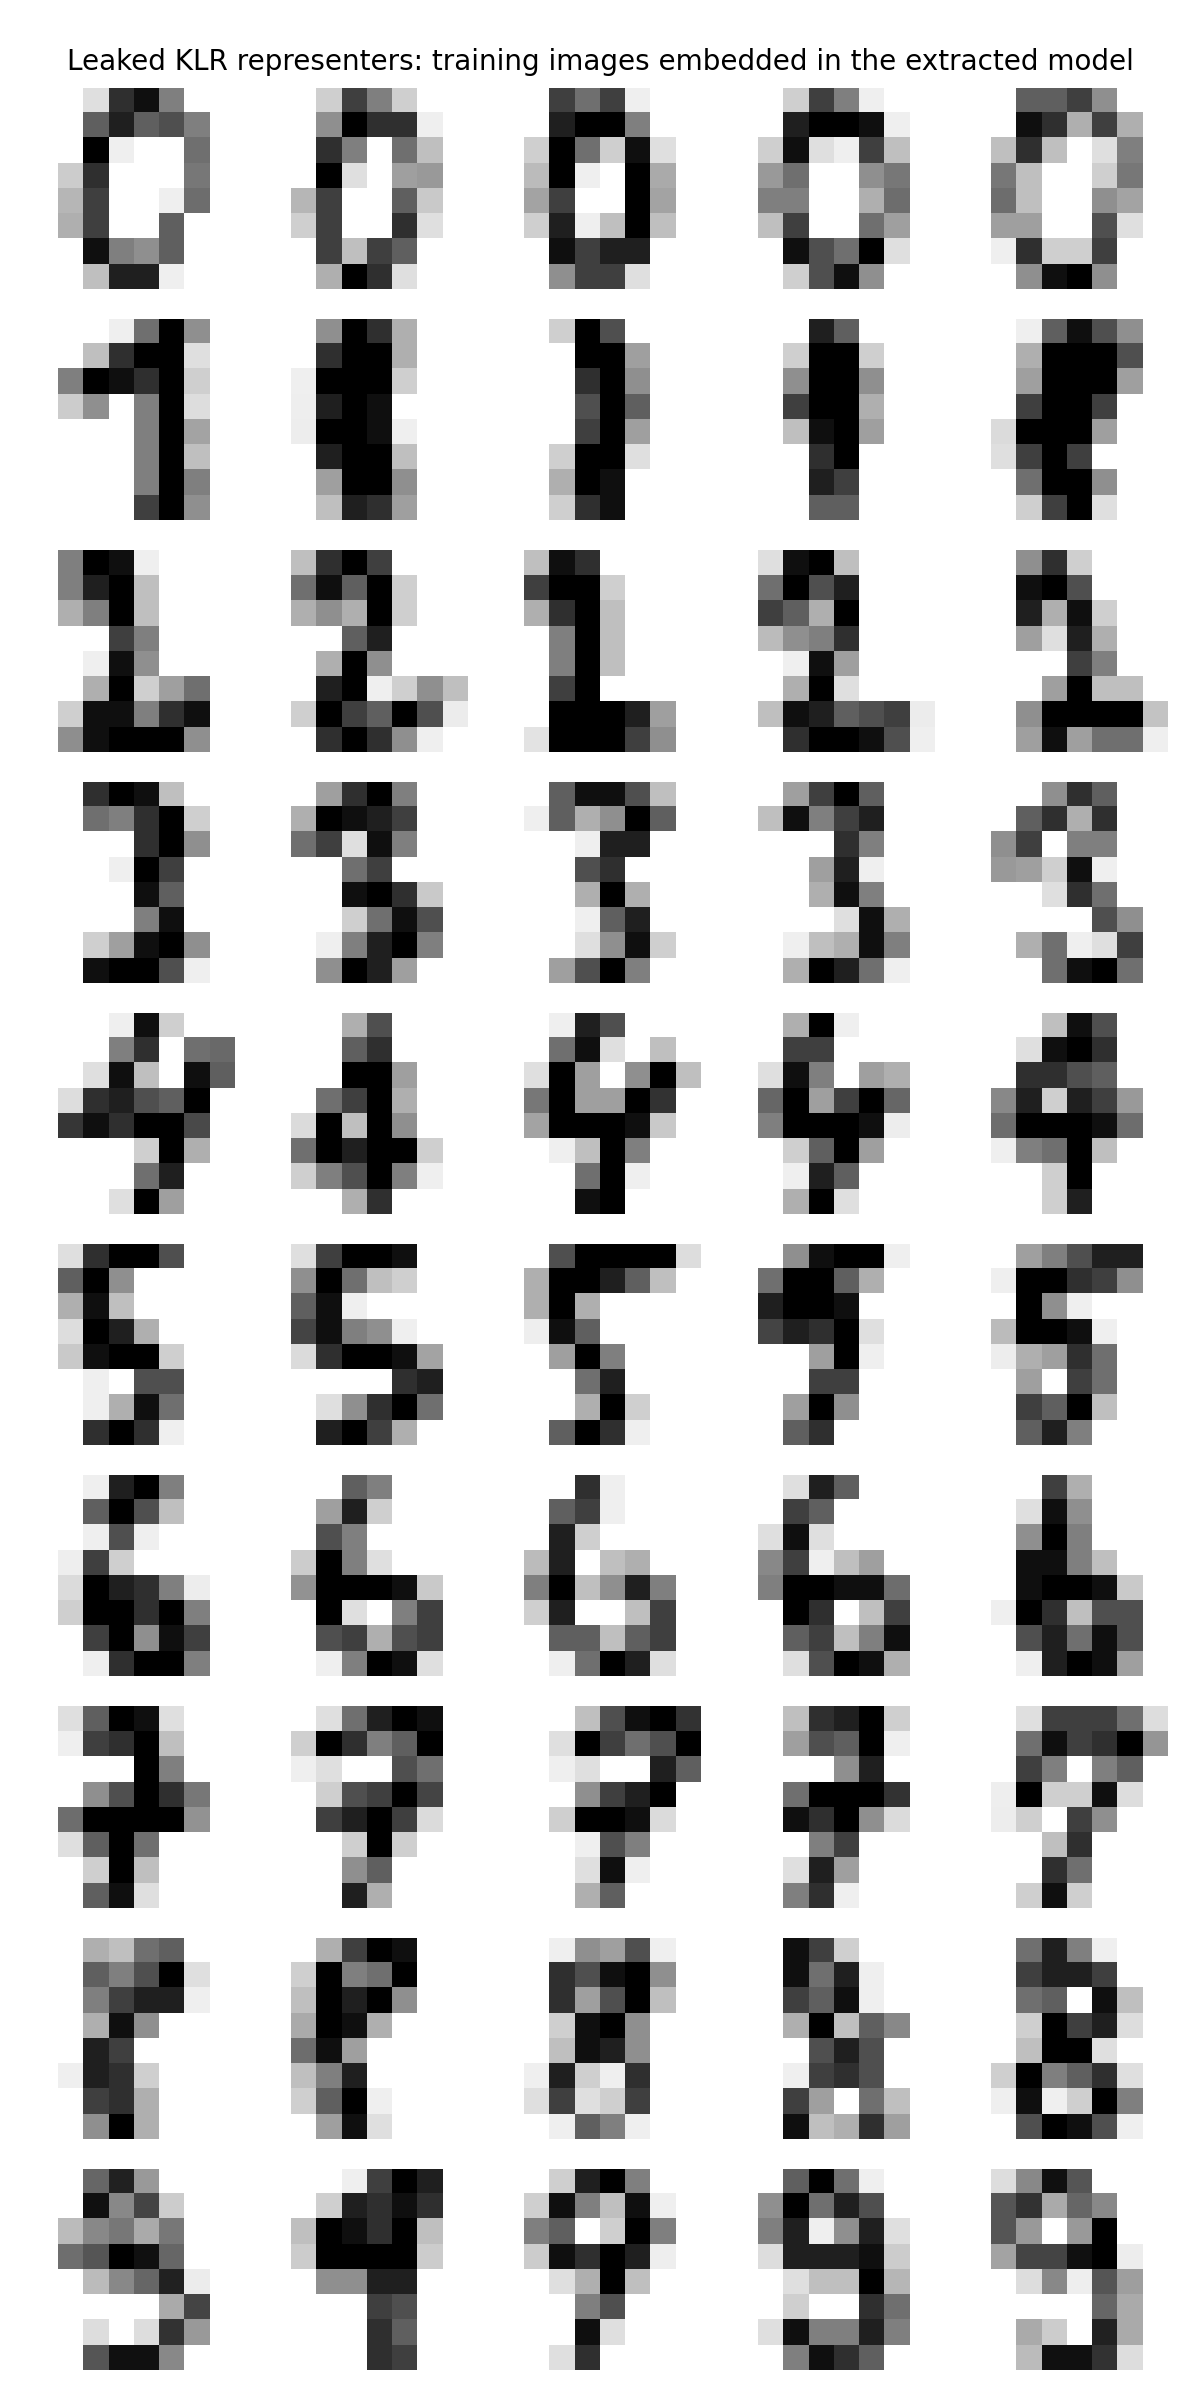
\includegraphics[height=0.68\textheight]{klr_leakage.png}
    \end{column}
  \end{columns}
\end{frame}

\begin{frame}{复现踩坑：这些可以作为组会补充}
  \small
  \begin{columns}[T,onlytextwidth]
    \begin{column}{0.48\textwidth}
      \begin{block}{工程环境}
        \begin{itemize}
          \item 原仓库：Python 2 + Theano + 旧 sklearn
          \item 新环境：Python 3.14 + sklearn 1.8
          \item sklearn 移除了 \code{multi\_class} 参数
          \item 解决：softmax 用新版默认 LR，OvR 显式套 \code{OneVsRestClassifier}
        \end{itemize}
      \end{block}
      \begin{block}{本机环境}
        \begin{itemize}
          \item Arch/PEP 668 禁止系统 pip 安装
          \item 使用 \code{python -m venv .venv}
          \item 用户级 \code{distutils-precedence.pth} 警告不影响运行
        \end{itemize}
      \end{block}
    \end{column}
    \begin{column}{0.48\textwidth}
      \begin{block}{算法实现}
        \begin{itemize}
          \item 决策树不能只看区间两端 leaf id
          \item 可能出现“两端同叶，中间另有叶”
          \item 连续阈值有 \code{<=} / \code{>} 边界问题
          \item 最终按“当前叶子的路径谓词”逐特征恢复
        \end{itemize}
      \end{block}
      \begin{block}{汇报时的表述}
        这次复现是“重写核心机制”，不是“跑通旧仓库”：算法思想稳定，但工程依赖和 API 会随时间变化。
      \end{block}
    \end{column}
  \end{columns}
\end{frame}

\begin{frame}{Takeaways}
  \begin{block}{我们复现到的核心结论}
    \begin{itemize}
      \item Confidence values 让 LR 提取从学习问题变成解方程问题
      \item 对多类 LR，约 1 query / parameter 即可达到近似完美一致
      \item Decision tree 可利用 leaf identity 做路径查找
      \item Label-only 能提高成本，但不能根除提取
      \item Kernel representer 模型存在训练数据泄露风险
    \end{itemize}
  \end{block}
  \begin{block}{当前复现限制}
    未复跑 AWS/BigML 在线实验；决策树和 KLR 是教学版；MLP、Lowd-Meek 完整实现可作为后续扩展。
  \end{block}
\end{frame}

\end{document}
